%%%%%%%%%%%%%%%%%%%%%%%%%%%%%%%%%%%%%%%%%%%%%%%%%%%%%%%%%%%%%%%%%%%%%%%%%%%%%%%%
%% Plantilla de memoria en LaTeX para la ETSIT - Universidad Rey Juan Carlos
%%
%% Por Gregorio Robles <grex arroba gsyc.urjc.es>
%%     Grupo de Sistemas y Comunicaciones
%%     Escuela Técnica Superior de Ingenieros de Telecomunicación
%%     Universidad Rey Juan Carlos
%% (muchas ideas tomadas de Internet, colegas del GSyC, antiguos alumnos...
%%  etc. Muchas gracias a todos)
%%
%% La última versión de esta plantilla está siempre disponible en:
%%     https://github.com/gregoriorobles/plantilla-memoria
%%
%% Para obtener PDF, ejecuta en la shell:
%%   make
%% (las imágenes deben ir en PNG o JPG)

%%%%%%%%%%%%%%%%%%%%%%%%%%%%%%%%%%%%%%%%%%%%%%%%%%%%%%%%%%%%%%%%%%%%%%%%%%%%%%%%

\documentclass[a4paper, 12pt]{book}
%\usepackage[T1]{fontenc}

\usepackage[a4paper, left=2.5cm, right=2.5cm, top=3cm, bottom=3cm]{geometry}
\usepackage{times}
\usepackage[utf8]{inputenc}
\usepackage[spanish]{babel} % Comenta esta línea si tu memoria es en inglés
\usepackage{url}
%\usepackage[dvipdfm]{graphicx}
\usepackage{graphicx}
\usepackage{float}  %% H para posicionar figuras
\usepackage[nottoc, notlot, notlof, notindex]{tocbibind} %% Opciones de índice
\usepackage{latexsym}  %% Logo LaTeX

\title{Memoria del Proyecto}
\author{Fernando Caballero Sánchez}

\renewcommand{\baselinestretch}{1.5}  %% Interlineado

\begin{document}

\renewcommand{\refname}{Bibliografía}  %% Renombrando
\renewcommand{\appendixname}{Apéndice}

%%%%%%%%%%%%%%%%%%%%%%%%%%%%%%%%%%%%%%%%%%%%%%%%%%%%%%%%%%%%%%%%%%%%%%%%%%%%%%%%
% PORTADA

\begin{titlepage}
\begin{center}
\begin{tabular}[c]{c c}
%\includegraphics[bb=0 0 194 352, scale=0.25]{logo} &
\includegraphics[scale=0.25]{img/logo_vect.png} &
\begin{tabular}[b]{l}
\Huge
\textsf{UNIVERSIDAD} \\
\Huge
\textsf{REY JUAN CARLOS} \\
\end{tabular}
\\
\end{tabular}

\vspace{3cm}

\Large
DOBLE LICENCIATURA EN INGENIERÍA DE TELECOMUNICACIÓN Y ADMINISTRACIÓN Y DIRECCIÓN DE EMPRESAS

\vspace{0.4cm}

\large
Curso Académico 2016/2017

\vspace{0.8cm}

Proyecto Fin de Carrera

\vspace{2.5cm}

\LARGE
MANTENIMIENTO Y SOPORTE DE UN DATAMART DE RIESGOS

\vspace{4cm}

\large
Autor : Fernando Caballero Sánchez \\
Tutor : Dr. Gregorio Robles
\end{center}
\end{titlepage}

\newpage
\mbox{}
\thispagestyle{empty} % para que no se numere esta pagina


%%%%%%%%%%%%%%%%%%%%%%%%%%%%%%%%%%%%%%%%%%%%%%%%%%%%%%%%%%%%%%%%%%%%%%%%%%%%%%%%
%%%% Para firmar
\clearpage
\pagenumbering{gobble}
\chapter*{}

\vspace{-4cm}
\begin{center}
\LARGE
\textbf{Proyecto Fin de Carrera}

\vspace{1cm}
\large
Mantenimiento y soporte de un Datamart de riesgos

\vspace{1cm}
\large
\textbf{Autor :} Fernando Caballero Sánchez \\
\textbf{Tutor :} Dr. Gregorio Robles Martínez

\end{center}

\vspace{1cm}
La defensa del presente Proyecto Fin de Carrera se realizó el día \qquad$\;\,$ de \qquad\qquad\qquad\qquad \newline de 2017, siendo calificada por el siguiente tribunal:


\vspace{0.5cm}
\textbf{Presidente:}

\vspace{1.2cm}
\textbf{Secretario:}

\vspace{1.2cm}
\textbf{Vocal:}


\vspace{1.2cm}
y habiendo obtenido la siguiente calificación:

\vspace{1cm}
\textbf{Calificación:}


\vspace{1cm}
\begin{flushright}
Fuenlabrada, a \qquad$\;\,$ de \qquad\qquad\qquad\qquad de 2017
\end{flushright}

%%%%%%%%%%%%%%%%%%%%%%%%%%%%%%%%%%%%%%%%%%%%%%%%%%%%%%%%%%%%%%%%%%%%%%%%%%%%%%%%
%%%% Dedicatoria

\chapter*{}
\pagenumbering{Roman} % para comenzar la numeracion de paginas en numeros romanos
\begin{flushright}
\textit{Dedicado a \\
mi familia y a mi mujer}
\end{flushright}

%%%%%%%%%%%%%%%%%%%%%%%%%%%%%%%%%%%%%%%%%%%%%%%%%%%%%%%%%%%%%%%%%%%%%%%%%%%%%%%%
%%%% Agradecimientos

\chapter*{Agradecimientos}
%\addcontentsline{toc}{chapter}{Agradecimientos} % si queremos que aparezca en el Índice
\markboth{AGRADECIMIENTOS}{AGRADECIMIENTOS} % encabezado 
Siempre es difícil acordarse de todas y cada una de las personas que merecen ser nombradas. Para evitar dejarme ningún nombre en el tintero, no puedo más que dar las gracias a todas y cada una de las personas con las que, de una forma u otra, he compartido momentos durante el paso por la universidad.

Sin embargo, hay personas que merecen una mención especial: papá, mamá y Cristina, gracias por aguantarme, animarme y apoyarme durante estos años. Papá, gracias por orientarme y aconsejarme con tu experiencia, hoy sí te lo puedo decir: tenías razón siempre. Mamá, gracias por tu constancia y tu paciencia infinita.

También se merece una mención especial Irene. Llevas a mi lado desde 2008 y me has acompañado en todos los momentos de mi vida desde entonces, tanto en lo académico como en lo personal. No puedo más que agradecerte tu apoyo incondicional y tu cariño.

Por supuesto, David gracias por estar ahí desde que empezamos esta doble licenciatura. Además de compañero, te considero amigo incondicional y hermano. Lo que la programación y las integrales han unido, nada lo puede separar.

Y para terminar con el ámbito personal, agradecer especialmente al pequeño grupo de \textit{Telecolades} y al resto de compañeros entre los que formamos el reducido grupo en los últimos años.

Me gustaría también agradecer a everis por ofrecerme la oportunidad de colaborar en uno de sus proyectos y por ser el punto de inicio de mi carrera profesional. Agradecer también al equipo liderado por Pedro Palacios por su tiempo dedicado a formarme en el ámbito del análisis de datos.

En el apartado más académico, agradecer a la Universidad Rey Juan Carlos y a todo su equipo docente el tiempo, energía y esfuerzo dedicados. Soy consciente del esfuerzo que os ha supuesto a todos los docentes el compaginar nuestra antigua titulación con los actuales grados, ofreciendo tutorías de manera altruista multiplicando vuestra carga de trabajo. Por todo ello, os doy las gracias.

Por último, me gustaría agradecer la infinita paciencia de mi tutor, Gregorio. Así mismo, como alumno de la Universidad Rey Juan Carlos, agradecerle su dedicación, pasión y entusiasmo como docente, derrochando alegría en todas y cada una de las clases que recuerdo.

%%%%%%%%%%%%%%%%%%%%%%%%%%%%%%%%%%%%%%%%%%%%%%%%%%%%%%%%%%%%%%%%%%%%%%%%%%%%%%%%
%%%% Resumen

\chapter*{Resumen}
%\addcontentsline{toc}{chapter}{Resumen} % si queremos que aparezca en el Índice
\markboth{RESUMEN}{RESUMEN} % encabezado

En la actualidad, el análisis de los datos generados en el entorno de una organización resulta vital para la toma de decisiones del negocio. Este análisis se lleva a cabo ya sea mediante simples cruces de datos o a través de complejos modelos estadísticos capaces de predecir la tendencia o comportamiento a futuro de los clientes.

En este contexto se desarrolla este proyecto, en el cual se analiza el concepto de \textit{Datamart}, así como las consideraciones y ejemplos útiles de cómo realizar su mantenimiento y soporte durante la operación del mismo. Así pues, el objetivo principal es el de conocer el funcionamiento de un Datamart, las tareas necesarias para dar soporte a su operativa y el mantenimiento del mismo.

Las principales tecnologías involucradas durante el proyecto han sido las bases de datos de Oracle y la programación de \textit{scripts} en PL/SQL, lenguaje propio de las bases de datos. Así mismo, el manejo de entornos UNIX a través de línea de comandos, así como la programación y manejo de \textit{Shell scripts}.

Este proyecto se ha realizado en colaboración con el área de \textit{Business Intelligence} de everis. Durante la colaboración, se delegaron en mí las tareas de mantenimiento y soporte de un Datarmart de riesgos, el cual se encontraba en entorno productivo dando servicio a cliente, haciéndome responsable del buen funcionamiento y la correcta ejecución de los procesos. 

%%%%%%%%%%%%%%%%%%%%%%%%%%%%%%%%%%%%%%%%%%%%%%%%%%%%%%%%%%%%%%%%%%%%%%%%%%%%%%%%
%%%% Resumen en inglés

\chapter*{Summary}
%\addcontentsline{toc}{chapter}{Summary} % si queremos que aparezca en el Índice
\markboth{SUMMARY}{SUMMARY} % encabezado

En la actualidad, el análisis de los datos generados en el entorno de una organización resulta vital para la toma de decisiones del negocio. Este análisis se lleva a cabo ya sea mediante simples cruces de datos o a través de complejos modelos estadísticos capaces de predecir la tendencia o comportamiento a futuro de los clientes.

En este contexto se desarrolla este proyecto, en el cual se analiza el concepto de \textit{Datamart}, así como las consideraciones y ejemplos útiles de cómo realizar su mantenimiento y soporte durante la operación del mismo. Así pues, el objetivo principal es el de conocer el funcionamiento de un Datamart, las tareas necesarias para dar soporte a su operativa y el mantenimiento del mismo.

Las principales tecnologías involucradas durante el proyecto han sido las bases de datos de Oracle y la programación de \textit{scripts} en PL/SQL, lenguaje propio de las bases de datos. Así mismo, el manejo de entornos UNIX a través de línea de comandos, así como la programación y manejo de \textit{Shell scripts}.

Este proyecto se ha realizado en colaboración con el área de \textit{Business Intelligence} de everis. Durante la colaboración, se delegaron en mí las tareas de mantenimiento y soporte de un Datarmart de riesgos, el cual se encontraba en entorno productivo dando servicio a cliente, haciéndome responsable del buen funcionamiento y la correcta ejecución de los procesos.


%%%%%%%%%%%%%%%%%%%%%%%%%%%%%%%%%%%%%%%%%%%%%%%%%%%%%%%%%%%%%%%%%%%%%%%%%%%%%%%%
%%%%%%%%%%%%%%%%%%%%%%%%%%%%%%%%%%%%%%%%%%%%%%%%%%%%%%%%%%%%%%%%%%%%%%%%%%%%%%%%
% ÍNDICES %
%%%%%%%%%%%%%%%%%%%%%%%%%%%%%%%%%%%%%%%%%%%%%%%%%%%%%%%%%%%%%%%%%%%%%%%%%%%%%%%%

% Las buenas noticias es que los Índices se generan automáticamente.
% Lo único que tienes que hacer es elegir cuáles quieren que se generen,
% y comentar/descomentar esa instrucción de LaTeX.

%%%% Índice de contenidos
\tableofcontents 
%%%% Índice de figuras
\cleardoublepage
%\addcontentsline{toc}{chapter}{Lista de figuras} % para que aparezca en el indice de contenidos
\listoffigures % indice de figuras
%%%% Índice de tablas
%\cleardoublepage
%\addcontentsline{toc}{chapter}{Lista de tablas} % para que aparezca en el indice de contenidos
%\listoftables % indice de tablas

%%%%%%%%%%%%%%%%%%%%%%%%%%%%%%%%%%%%%%%%%%%%%%%%%%%%%%%%%%%%%%%%%%%%%%%%%%%%%%%%
%%%%%%%%%%%%%%%%%%%%%%%%%%%%%%%%%%%%%%%%%%%%%%%%%%%%%%%%%%%%%%%%%%%%%%%%%%%%%%%%
% INTRODUCCIÓN %
%%%%%%%%%%%%%%%%%%%%%%%%%%%%%%%%%%%%%%%%%%%%%%%%%%%%%%%%%%%%%%%%%%%%%%%%%%%%%%%%

\cleardoublepage
\chapter{Introducción}
\label{sec:intro} % etiqueta para poder referenciar luego en el texto con ~\ref{sec:intro}
\pagenumbering{arabic} % para empezar la numeración de página con números

\section{Contexto}
\label{sec:Contexto}

En la actualidad, el área de Inteligencia de Negocio o \textit{Business Intelligence} (BI) ha adquirido una gran relevancia para las empresas. Esto es así debido a la elevada capacidad tanto de almacenamiento como de procesamiento de datos, los cuales se desechaban por resultar demasiado costoso su almacenamiento y/o tratamiento. A través de un adecuado tratamiento de toda esa información, las organizaciones son capaces de tomar decisiones de negocio de la forma más acertada posible: descifrando tendencias, segmentando mercados y teniendo un mayor conocimiento de la actuación de la organización en un determinado mercado.

El principal objetivo de la inteligencia de negocio consiste en hacer de los datos información de valor y conocimiento, de manera que la toma de decisiones pueda sustentarse en el procesado de esos datos.

Son varios los medios especializados y estudios \cite{BI_tendencies1,BI_tendencies2,BI_tendencies3,BI_tendencies4} que indican que aún queda mucho camino por recorrer en el mundo del \textit{Business Intelligence}. Por un lado, aumentará la demanda de herramientas que permitan acceder a gráficos más potentes y con capacidades creativas más avanzadas. Además, se tenderá a un modelo de BI de autoservicio, en el que las propias áreas de negocio accederán a la información y llevarán a cabo las transformaciones y procesado necesario.

Así pues, este proyecto se desarrolla en este contexto de especial incremento del interés por parte de las organizaciones en el \textit{Business Intelligence} como palanca para llevar a cabo su transformación digital.

\section{Motivación}
\label{sec:motivacion}
La motivación por realizar este proyecto surge con la oportunidad de llevar a cabo una colaboración con una consultora en el ámbito del \textit{Business Intelligence}. Tras analizar las posibilidades que ofrecen las empresas de consultoría en cuanto a un aprendizaje rápido y con una clara orientación a objetivos y a la satisfacción de las necesidades del cliente, considero que es una gran oportunidad para dar los primeros pasos de la carrera profesional. A esto se le une la pasión por la tecnología y los ordenadores que siempre he tenido, cultivada a través de todos estos años en la universidad, y el gran \textit{boom} que en este momento presenta el análisis de datos masivos.

\section{Dedicación}
\label{sec:dedicacion}
Como se indica en el apartado anterior, este proyecto se ha realizado en colaboración con el área de \textit{Business Intelligence} de everis. Esta colaboración tuvo una duración de siete meses con una dedicación de jornada completa, durante la cual recibí formación del equipo de trabajo del proyecto del Datamart de riesgos para abordar las tareas que me fueron asignadas de manera adecuada. 


\section{Estructura de esta memoria}
\label{sec:estructura}
El objetivo de este apartado es facilitar la lectura y uso del presente documento, para lo cual se presenta a continuación la estructura del mismo, detallando qué contenido se podrá encontrar en cada capítulo:

\begin{enumerate}
	\item \textbf{Introducción.}\par
	Se introduce el contexto en el que se ha llevado a cabo a cabo el proyecto, explicando la situación actual, además de su justificación. Así mismo, se explica la motivación que surge para la realización del proyecto. Por último, en este capítulo se encuentra este resumen de la estructura. 
	
	\item \textbf{Objetivos.}\par
	En este segundo capítulo se recogen tanto los objetivos generales del proyecto, como los objetivos específicos que, en un principio, se pretenden abordar.
	
	\item \textbf{Estado del arte.}\par
	Se presentan tanto las tecnologías empleadas para llevar a cabo el proyecto, como el estado actual de las mismas. De manera adicional, se explica la contribución de cada una de las tecnologías en el proyecto y una pequeña introducción para su configuración.
		
	\item \textbf{Diseño e implementación.}\par
	En este capítulo se detalla el uso que se hace de las tecnologías explicadas en el capítulo anterior. Se analiza en detalle la arquitectura y diseño del Datamart, así como las principales tareas necesarias y consideraciones más relevantes para mantener y dar soporte a un Datamart.
	
	\item \textbf{Resultados.}\par
	Se hace mención a los resultados obtenidos fruto del trabajo llevado a cabo durante el Proyecto.
	
	\item \textbf{Conclusiones.}\par
	En este último capítulo se lleva a cabo una reflexión a alto nivel sobre el recorrido del proyecto. En primer lugar, se analiza el nivel de consecución de los objetivos planteados. Por otro lado, se expondrán los conocimientos adquiridos durante la formación en la Doble Licenciatura en Ingeniería de Telecomunicación y Administración y Dirección de Empresas en la Universidad Rey Juan Carlos y aplicados durante la realización del presente Proyecto Final de Carrera. Así mismo, se indicarán los conocimientos y habilidades adquiridas durante la realización del Proyecto. Por último, se mencionan una serie de recomendaciones acerca de los próximos pasos que se podrían abordar en el Proyecto.
	
\end{enumerate}


%%%%%%%%%%%%%%%%%%%%%%%%%%%%%%%%%%%%%%%%%%%%%%%%%%%%%%%%%%%%%%%%%%%%%%%%%%%%%%%%
%%%%%%%%%%%%%%%%%%%%%%%%%%%%%%%%%%%%%%%%%%%%%%%%%%%%%%%%%%%%%%%%%%%%%%%%%%%%%%%%
% OBJETIVOS %
%%%%%%%%%%%%%%%%%%%%%%%%%%%%%%%%%%%%%%%%%%%%%%%%%%%%%%%%%%%%%%%%%%%%%%%%%%%%%%%%

\cleardoublepage
\chapter{Objetivos}
\label{chap:objetivos}

\section{Objetivo general}
\label{sec:objetivo-general}
El objetivo principal de este proyecto es el de obtener los conocimientos acerca del funcionamiento de un Datamart, así como las tareas necesarias para dar soporte a su operativa y el mantenimiento del mismo.

\section{Objetivos específicos}
\label{sec:objetivos-especificos}
Para dar respuesta al objetivo principal, se pueden enumerar otra serie de objetivos específicos que han de ser cubiertos a lo largo del proyecto y entre los que se encuentran las tareas que fueron de mi responsabilidad durante la colaboración:

\begin{itemize}
	\item Conocer la arquitectura y la relación entre los diferentes sistemas de información involucrados.
	
	\item Monitorizar la ejecución de los procesos del Datamart de riesgos con el objetivo de garantizar que no se producen bloqueos en el Datamart.
	
	\item Optimizar la ejecución de los procesos del Datamart de riesgos.
	
	\item Asegurar el correcto funcionamiento de la máquina que soporta el Datamart de riesgos.
	
	\item Ejecutar procesos bajo demanda, asegurando la recepción de los datos necesarios así como el adecuado formato de los mismos.
	
	\item Realizar análisis de datos e informes y automatizarlos en la medida de lo posible.
\end{itemize}

%\section{Planificación temporal}
%\label{sec:planificacion-temporal}



%%%%%%%%%%%%%%%%%%%%%%%%%%%%%%%%%%%%%%%%%%%%%%%%%%%%%%%%%%%%%%%%%%%%%%%%%%%%%%%%
%%%%%%%%%%%%%%%%%%%%%%%%%%%%%%%%%%%%%%%%%%%%%%%%%%%%%%%%%%%%%%%%%%%%%%%%%%%%%%%%
% ESTADO DEL ARTE %
%%%%%%%%%%%%%%%%%%%%%%%%%%%%%%%%%%%%%%%%%%%%%%%%%%%%%%%%%%%%%%%%%%%%%%%%%%%%%%%%

\cleardoublepage
\chapter{Estado del arte}

\section{Arquitectura y diseño de un Datamart} 
\label{sec:datamart}
El principal motivo por el que una organización necesita disponer de un Data Warehouse surge debido a que los datos clave de toda la organización se encuentran fragmentados a lo largo de múltiples y dispares aplicativos, ejecutándose en diferentes plataformas y en distintas localizaciones físicas. Esta situación no es favorable para una buena toma de decisiones. Además, cuando existe redundancia de datos en múltiples bases de datos, la calidad de los mismos suele tender a deteriorarse.

Por otro lado, las bases de datos operacionales están diseñadas para operar en los sistemas y recibir los datos de los mismos, por lo que no son adecuadas para llevar a cabo consultas y analíticas on-line.

Los entornos de Business Intelligence se pueden basar en diferentes arquitecturas, dependiendo en las necesidades específicas del negocio. El modelo que se muestra en la siguiente figura es el \textit{hub-and-spokes}, siendo el más popular y el que se usa en muchas organizaciones.

\begin{figure}
   \centering
   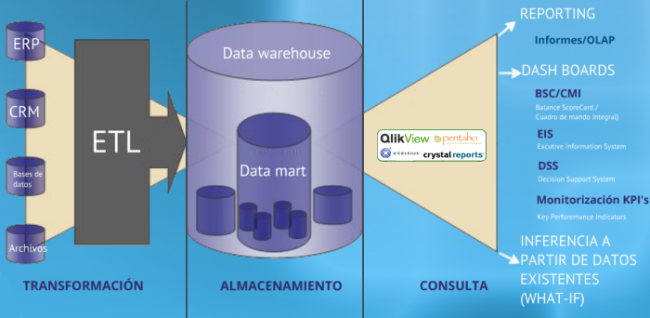
\includegraphics[width=14cm, keepaspectratio]{img/modelo_Datamart}
   \caption{Modelo Datamart hub-and-spokes}
   \label{fig:modelo_Datamart}
\end{figure}

El proceso que siguen los datos en este modelo es el siguiente: los datos se mueven desde las bases de datos de los sistemas operacionales hacia la zona de \textit{staging} del Data Warehouse, donde se preparan y modifican los datos para ser almacenados en el Data Warehouse. Finalmente, esos datos preparados se envían hacia los diferentes Data Marts que la organización haya definido.

La tecnología o proceso que se emplea para mover los datos en esta arquitectura se denomina ETL (por sus siglas en inglés ``Extract, Transform and Load"). Se emplea para transferir datos desde las aplicaciones operacionales a la zona de \textit{staging} del Data Warehouse, desde esta al Data Warehouse, y desde este último a cada uno de los Data Marts.

Mediante el proceso de ETL los datos se extraen, se transforman los valores de los datos inconsistentes, se limpian los datos mal formados, se filtran los datos y se cargan en la base de datos objetivo. La programación temporal de los trabajos de ETL es crítica, así como la tolerancia a errores: en caso de fallo de uno de estos trabajos, el resto debería responder de manera apropiada.

El área de \textit{staging} del Data Warehouse es donde se copian los datos de los sistemas de origen de manera temporal. Este paso es fundamental en muchas arquitecturas de Data Warehouse para coordinar los tiempos entre todos los sistemas. De manera resumida, todos los datos que se necesitan deben estar disponibles al mismo tiempo antes de ser integrados en el Data Warehouse y, debido a, entre otras casos, los diferentes ciclos del negocio, los ciclos de procesamiento de datos en los sistemas de origen y las limitaciones de recursos hardware y red, no es factible extraer todos los datos de todas las bases de datos operacionales exactamente al mismo tiempo. Por ejemplo, puede ser razonable extraer la información de ventas diaria, sin embargo, extracciones diarias pueden no ser adecuadas para la información financiera que requiere un proceso de reconciliación a mes cerrado. Por último, es importante tener en cuenta que no todas las organizaciones necesitan un área de \textit{staging} en su Data Warehouse, ya que para muchos negocios es factible usar ETL para copiar directamente la información de las bases de datos operacionales al Data Warehouse.

El objetivo del Data Warehouse en toda la arquitectura es integrar la información corporativa. En este sentido, será el Data Warehouse el que contenga la “única versión de la verdad” para la organización, que habrá sido cuidadosamente construida a partir de la información almacenada en diferentes bases de datos operacionales. La cantidad de información que se llega a almacenar en un Data Warehouse es masiva, debido a que los datos se almacenan en un nivel de detalle muy granular. Por ejemplo, cada venta que ha tenido lugar en una organización se almacena y relaciona, permitiendo llevar a cabo agregados, agrupaciones, filtrados y demás operaciones en una cantidad casi ilimitada de formas.

Un aspecto a destacar es que, a diferencia de lo que se suele pensar de manera generalizada, el Data Warehouse no contiene toda la información que existe en una organización. El objetivo de un Data Warehouse es proporcionar métricas clave para el negocio que sean necesarias y útiles para la toma de decisión táctica y estratégica de la organización.

Debido al gran volumen de información que almacena un Data Warehouse, las personas que toman decisiones y necesitan las métricas no acceden a este Data Warehouse directamente. Esto lo hacen a través de varias herramientas “front-end” que leen datos de los Data Marts específicos de cada área de negocio o temática.

Los trabajos de ETL extraen la información del Data Warehouse y pueblan el/los Data Marts de la organización para su uso por parte de los grupos que toman las decisiones dentro de las organizaciones. Los Data Marts pueden ser dimensionales (esquemas en estrella) o relacionales, en función de como se necesite consumir la información y de qué herramienta de “front-end” se emplee para presentar la información.

Cada Data Mart puede contener diferentes combinaciones de tablas, columnas y filas del Data Warehouse de la organización. Por ejemplo, una unidad de negocio o grupo de usuarios que no necesita datos históricos puede requerir únicamente las transacciones del año en curso, o el área de recursos humanos puede necesitar ver todos los detalles de todos los empleados, mientras que información como el salario o dirección de casa puede no ser apropiada para un Data Mart orientado al área de ventas \cite{dwh1,dwh2,dwh3,dwh4,dwh5,dwh6,dwh7,dwh8}.

\section{Cliente VPN de Cisco}
\label{sec:Cisco_VPN}

El cliente VPN de Cisco es una herramienta del proveedor Cisco que permite configurar una red VPN. Actualmente se encuentra obsoleta y sin soporte por parte del fabricante \cite{cisco01:_cisco_vpn_client01}. A través de Cisco VPN Cliente se crea una conexión segura sobre Internet entre los ordenadores y las máquinas donde residen tanto los datos del Datamart como la ejecución de los diferentes procesos propios del Datamart de Riesgos. Por lo tanto, esta herramienta permite acceder a la red privada de las máquinas del Datamart como si nos encontrásemos físicamente en la red \cite{cisco02:_cisco_vpn_client02}.

Una vez instalada la herramienta es necesario configurarla, agregando la conexión con los parámetros facilitados por el cliente. Para garantizar una conexión segura, el cliente proporciona los certificados necesarios, los cuales habrá que seleccionar también en el cliente VPN \cite{deal2005complete}.

A continuación, se muestra una captura de pantalla de la herramienta Cisco VPN Client donde se lleva a cabo la configuración de la conexión.

\begin{figure}
   \centering
   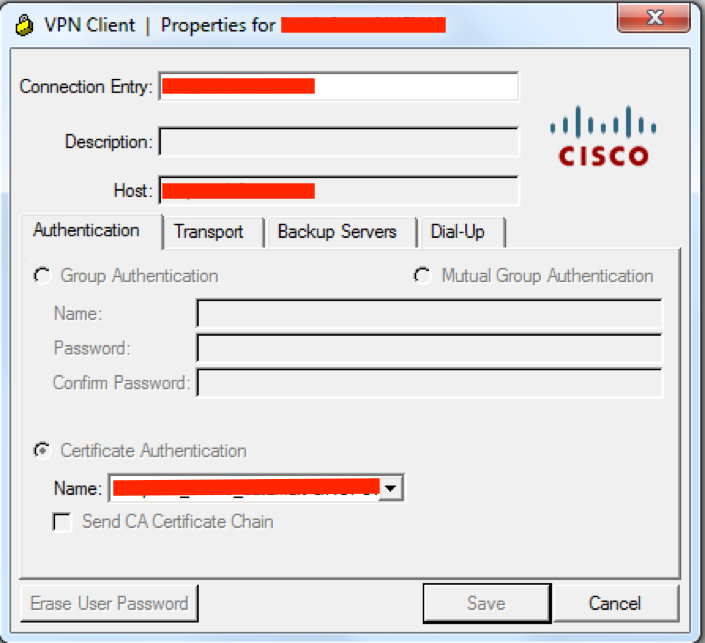
\includegraphics[width=12cm, keepaspectratio]{img/ciscovpnclient}
   \caption{Pantalla de configuración del Cliente VPN de Cisco}
   \label{fig:CiscoVpnClient_Config}
\end{figure}

\section{Oracle}
\label{sec:Oracle}
Oracle Database es un sistema de gestión de base de datos de tipo objeto-relacional (ORDBMS, por el acrónimo en inglés de Object-Relational Data Base Management System), desarrollado por Oracle Corporation. Durante el desarrollo de este proyecto se usa la versión 11.2.0 de Oracle Database \cite{Ashdown_oracle}.

Cabe señalar que el lenguaje usado para la gestión de la base de datos de Oracle es el Structured Query Language o SQL, así como la extensión procedimental PL/SQL para Oracle \cite{oracle02}:
\begin{itemize}
	\item SQL (por sus siglas en inglés \textit{Structured Query Language}) es un lenguaje declarativo basado en conjuntos que proporciona una interfaz a una RDBMS, como por ejemplo a la base de datos de Oracle. De manera contraria a otros lenguajes procedimentales (como por ejemplo C) que describen como se deben hacer las cosas, SQL es no-procedimental y simplemente describe qué se debe hacer. Los usuarios/programadores especifican el resultado que quieren obtener, no cómo obtenerlo.
	
Todas las operaciones sobre los datos almacenados en una base de datos bajo Oracle se realizan mediante sentencias SQL, también conocidas como \textit{queries}. Por ejemlpo, se emplea SQL para crear tablas, así como para consultar y modificar la información contenida en esas tablas.
	\item PL/SQL es una extensión procedimental para Oracle SQL. PL/SQL está integrado con las bases de datos de Oracle, permitiendo a los usuarios emplear todas las instrucciones SQL, funciones y tipos de datos de las bases de datos de Oracle. Así, es posible usar PL/SQL para controlar el flujo de un programa SQL, utilizar variables, y escribir procedimientos que manejen los errores.
	
El principal beneficio de PL/SQL es la capacidad de almacenar toda la lógica de la aplicación en la propia base de datos. Un procedimiento o una función es un objeto del esquema que está formado por una serie de instrucciones SQL y por construcciones PL/SQL, agrupadas y almacendas en la base de datos, ejecutándose como una unidad para resolver un problema específico o para realizar una serie de tareas relacionadas. El mayor beneficio de la programación del lado del servidor es que la funcionalidad incorporada al aplicativo se puede desplegar en cualquier lugar.
\end{itemize}

\section{PuTTY}
\label{sec:PuTTY}
PuTTY es una herramienta de software libre cuya misión es crear un terminal UNIX en entorno Windows. Esta herramienta la desarrolló originalmente Simon Tatham para plataformas Windows, aunque a día de hoy es soportado por voluntarios y se está trabajando en clientes para sistemas operativos Mac OS \cite{putty1,putty2,putty3}.

En este Proyecto, PuTTY se usa para abrir en los ordenadores desde donde se realiza el soporte y mantenimiento del Datamart un terminal UNIX conectado a través de SSH a las máquinas que alojan físicamente este Datamart de Riesgos.

En la figura~\ref{fig:PuTTY_Config} se muestra la pantalla de configuración de PuTTY, donde será necesario introducir los parámetros correspondientes para conectar con las máquinas del Datamart, una vez conectados a la red privada a través del cliente VPN.

\begin{figure}
   \centering
   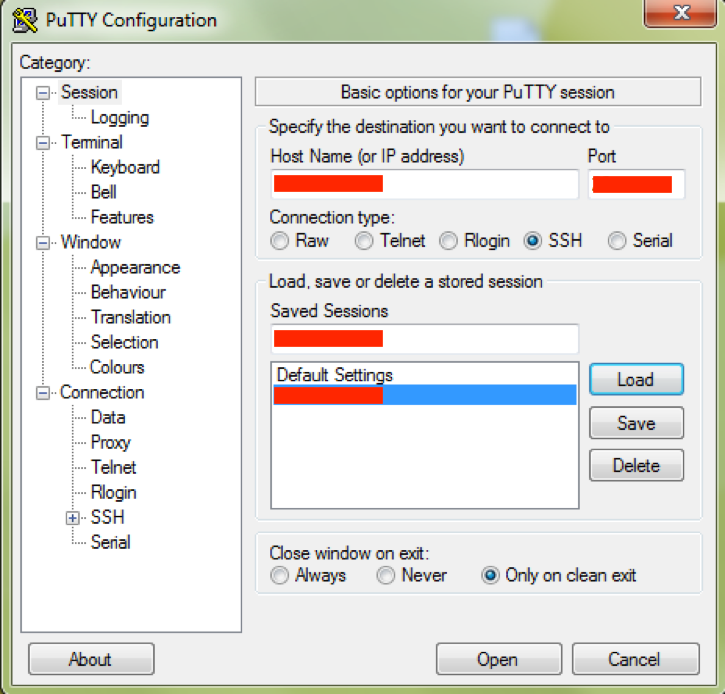
\includegraphics[width=12cm, keepaspectratio]{img/puttyconfig}
   \caption{Pantalla de configuración de PuTTY}
   \label{fig:PuTTY_Config}
\end{figure}

\section{Toad para Oracle}
\label{sec:Toad para Oracle}
Toad para Oracle es una herramienta que permite asegurar la máxima productividad en el desarrollo y administración de bases de datos Oracle, permitiendo reducir el tiempo y esfuerzo necesarios para desarrollar, administrar y mantener bases de datos de Oracle \cite{toad1}.

En la figura~\ref{fig:Toad_Config} se muestra una captura de pantalla de Toad for Oracle donde se lleva a cabo la configuración de los diferentes entornos (Desarrollo, Preproducción y Producción).

\begin{figure}
   \centering
   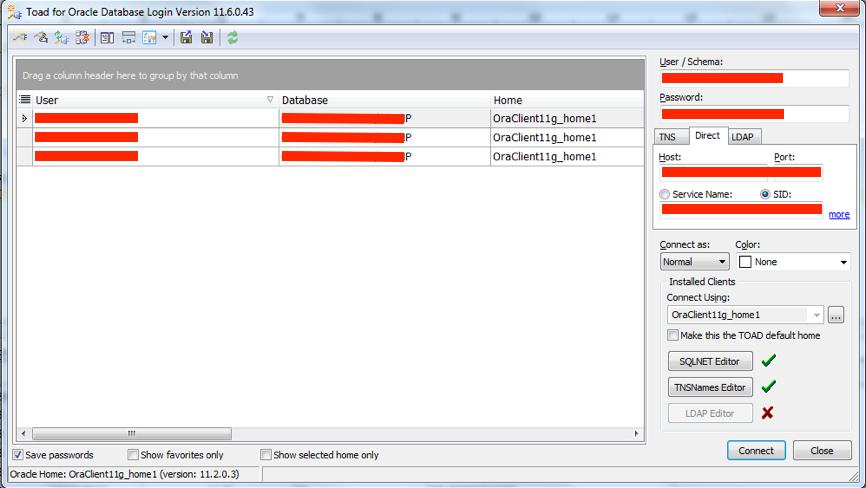
\includegraphics[width=12cm, keepaspectratio]{img/toadconfig}
   \caption{Pantalla de configuración de Toad para Oracle}
   \label{fig:Toad_Config}
\end{figure}

\section{FileZilla}
\label{sec:FileZilla}
FileZilla es una solución FTP de código abierto y software libre distribuido de manera gratuita bajo la Licencia Pública General GNU. Este software dispone tanto de cliente como de servidor, sin embargo, para el objeto de este Proyecto se usa únicamente el cliente FTP \cite{filezilla1}.

El cliente FTP permite la transferencia entre dos máquinas, en el caso de este Proyecto se conecta el cliente FTP a las máquinas donde reside el Datamart con el objetivo de administrar el sistema de ficheros desde entorno Windows desde la interfaz gráfica que proporciona el Cliente FTP de FileZilla. Para su correcto funcionamiento, es necesario configurar los parámetros correspondientes a la IP de la máquina remota, así como el usuario y contraseña \cite{filezilla2}.

En la figura~\ref{fig:FileZilla_Config} se presenta una captura de pantalla de la página de configuración del Cliente FTP de FileZilla.

\begin{figure}
   \centering
   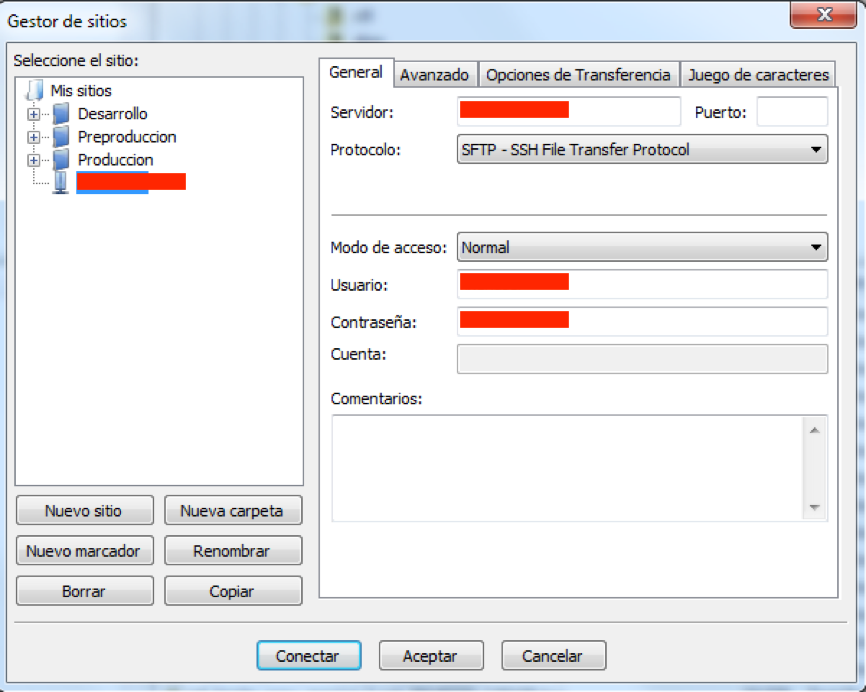
\includegraphics[width=12cm, keepaspectratio]{img/filezillaconfig}
   \caption{Pantalla de configuración del cliente de FileZilla}
   \label{fig:FileZilla_Config}
\end{figure}

\section{ODBC}
\label{sec:ODBC}
Por último, en la realización de este proyecto también es necesario disponer de ODBC configurado con el fin de llevar a cabo análisis de datos y actualización de informes ejecutados a través de Microsoft Excel \cite{microsoft_odbc}.

Open DataBase Connectivity (ODBC, por sus siglas) es un estándar de acceso a las bases de datos desarrollado por SQL Access Group. El objetivo de ODBC es hacer posible el acceso a cualquier dato desde cualquier aplicación, sin importar qué sistema de gestión de bases de datos almacene los datos \cite{alexandruaccess,odbc}.

Para configurar ODBC iremos al Administrador de orígenes de datos y en la pestaña “DNS de sistema” agregaremos tantos orígenes de datos como entornos o esquemas tengamos.

\section{Python}
\label{sec:Python}
Python es un lenguaje de programación de código abierto o “open-source” que cuenta con la licencia Python Software Foundation License, compatible con la Licencia pública general de GNU. La filosofía de Python hace hincapié en una sintaxis que favorece que el código sea legible, principal característica de este lenguaje de programación. Otras características que hacen de Python un lenguaje de programación muy versátil son las siguientes \cite{python01,python02,python03}:

\begin{itemize}
	\item Es un lenguaje de programación multiparadigma. Esto quiere decir que, más que forzar a los encargados del desarrollo del software a adoptar un estilo particular de programación, permite varios estilos: programación orientada a objetos, programación imperativa y programación funcional.

	\item Por otro lado, se trata de un lenguaje interpretado, es decir, no necesita compilación, con lo que la máquina es capaz de ejecutar la sucesión de instrucciones sin traducción previa. Esto hace que cualquier código sea independiente de las características concretas de la máquina o sistema operativo y, por tanto, es portable.

	\item Por último, Python usa tipado dinámico: una misma variable puede tomar valores de distinto tipo en diferentes momentos de la ejecución del código.
\end{itemize}

\section{Shell Scripts}
\label{sec:Shell_Scripts}
Los Shell Scripts contienen una serie de comandos de la Shell de Unix que, en la mayor parte de los que se usan en este proyecto, llevan a cabo una serie de operaciones sobre los ficheros y recopilan los parámetros necesarios para la ejecución del SQL correspondiente. Por ello, juegan un papel fundamental en este proyecto, ya que todos los procesos que se ejecutan para llevar a cabo las tareas propias del Datamart de Riesgos se lanzan a través de scripts. Un Shell script es un programa diseñado para ser ejecutado por la Shell de Unix, el intérprete de línea de comandos \cite{kernighan1984unix}.

%%%%%%%%%%%%%%%%%%%%%%%%%%%%%%%%%%%%%%%%%%%%%%%%%%%%%%%%%%%%%%%%%%%%%%%%%%%%%%%%
%%%%%%%%%%%%%%%%%%%%%%%%%%%%%%%%%%%%%%%%%%%%%%%%%%%%%%%%%%%%%%%%%%%%%%%%%%%%%%%%
% DISEÑO E IMPLEMENTACIÓN %
%%%%%%%%%%%%%%%%%%%%%%%%%%%%%%%%%%%%%%%%%%%%%%%%%%%%%%%%%%%%%%%%%%%%%%%%%%%%%%%%

\cleardoublepage
\chapter{Diseño e implementación}

Este capítulo contiene la parte principal del proyecto, ya que describe el diseño y funcionamiento del Datamart, las tareas principales llevadas a cabo en el soporte y mantenimiento del mismo, así como errores más comunes en su funcionamiento y las metodologías para solventarlos.

\section{Diseño general} 
\label{sec:diseno}
El Datamart de riesgos se divide en dos partes: operacional y analítico. En la parte del operacional se lleva a cabo el tratamiento de información y generación de informes relativos a los datos diarios. Por otro lado, en el analítico se lleva a cabo la manipulación de la información relativa a los ciclos de facturación o mensual.

El operacional del Datamart se procesa de manera diaria en un esquema propio de la base de datos. Hay que tener en cuenta que existe cierta información que se recibe y procesa varias veces al día, como es el caso de la información de consumos recibida desde Arbor. Las fuentes de entrada del sistema operacional son, en esencia, las siguientes:
\begin{itemize}
	\item Clarify: información relativa a la cartera de clientes. Desde Clarify se reciben una vez al día diferentes ficheros, entre ellos: clientes, cuentas, servicios, descuentos, límites, restricciones, promociones, … En la tabla de la figura~\ref{fig:entidades1} se muestran los ficheros que se reciben, así como la periodicidad, el volumen de registros y tamaño estimados.

	\begin{figure}
	  \centering
	  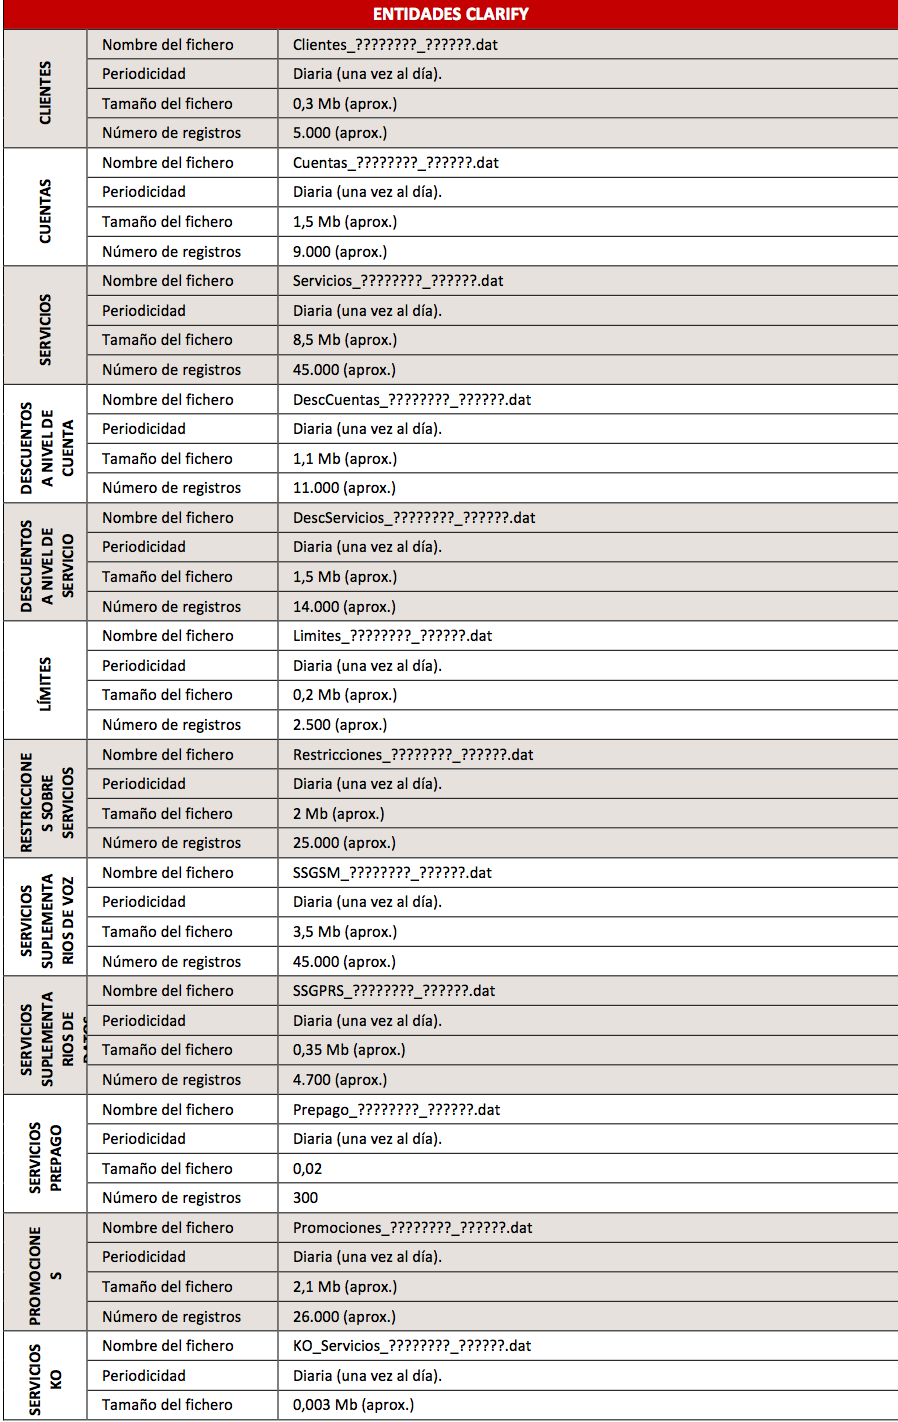
\includegraphics[width=14cm, keepaspectratio]{img/entidades1}
	  \caption{Entidades Clarify}
	  \label{fig:entidades1}
	\end{figure}
	
	\item Spirit: este sistema es, básicamente, el mismo que Clarify donde se está migrando toda la información. Por lo tanto, para tener toda la información de la cartera de clientes completa es necesario tratar datos que provienen de Spirit. Los ficheros recibidos son equivalentes a los de Clarify y también se reciben una vez al día. En la tabla de la figura~\ref{fig:entidades2} se muestran los detalles de los ficheros recibidos desde Spirit.

	\begin{figure}
	  \centering
	  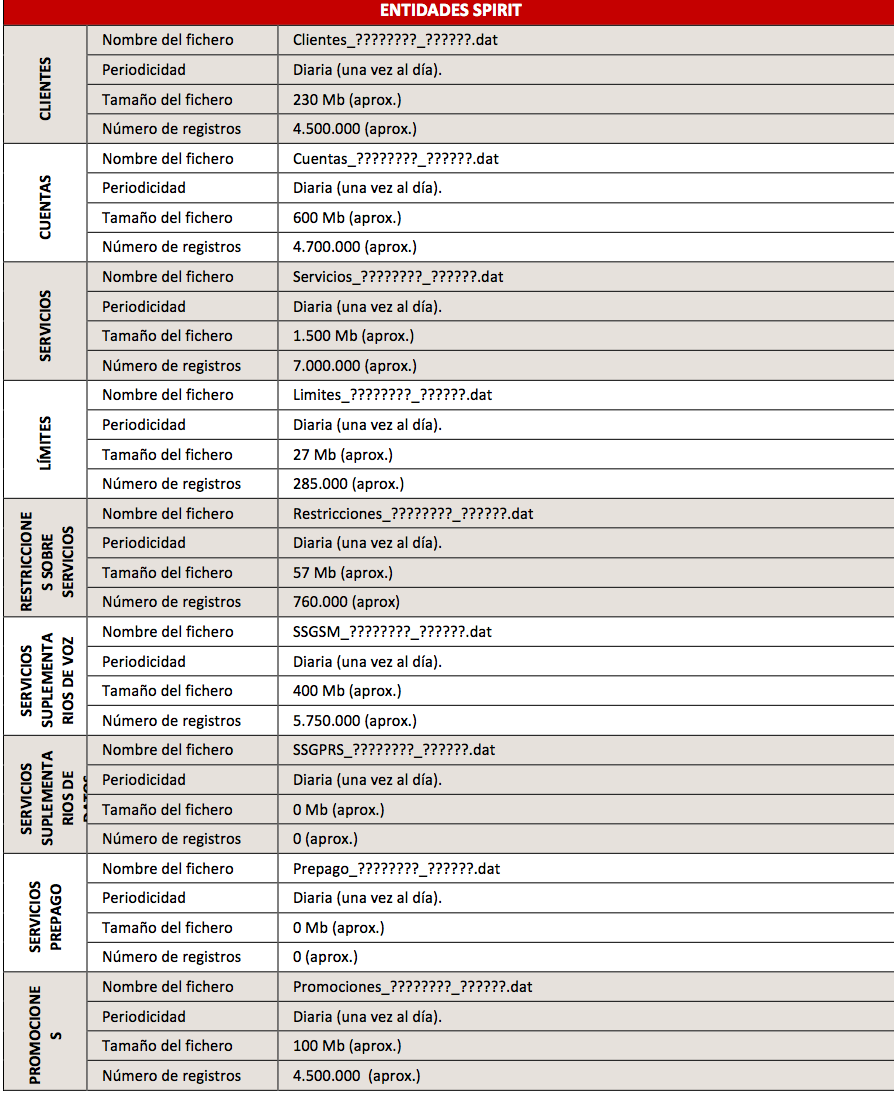
\includegraphics[width=14cm, keepaspectratio]{img/entidades2}
	  \caption{Entidades Spirit}
	  \label{fig:entidades2}
	\end{figure}
	
	\item Arbor: desde el sistema Arbor se recibe la información de consumo de los clientes. Esta información se recibe y procesa cada dos horas. En la tabla de la figura~\ref{fig:entidades3} se muestran los detalles de los ficheros recibidos desde Arbor.

	\begin{figure}
	  \centering
	  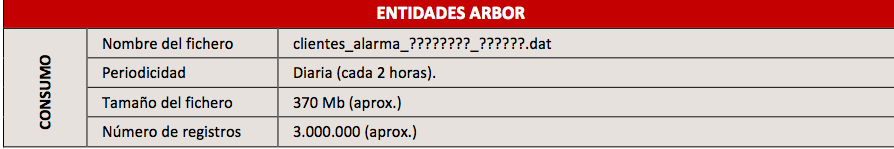
\includegraphics[width=14cm, keepaspectratio]{img/entidades3}
	  \caption{Entidades Arbor}
	  \label{fig:entidades3}
	\end{figure}
	
	\item CRM: desde CRM se recibe la información de cualquier contacto que tienen los calls centers con los clientes. Se reciben los ficheros una vez al día. En la tabla de la figura~\ref{fig:entidades4} se muestran los detalles de los ficheros recibidos.

	\begin{figure}
	  \centering
	  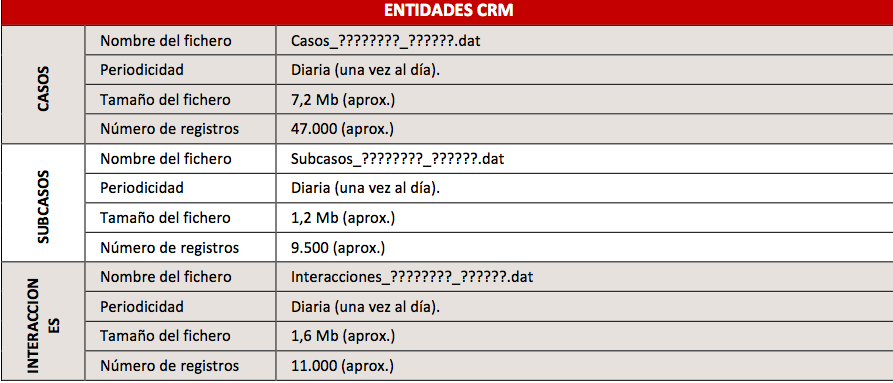
\includegraphics[width=14cm, keepaspectratio]{img/entidades4}
	  \caption{Entidades CRM}
	  \label{fig:entidades4}
	\end{figure}

	\item DWH: desde el Data Warehouse se reciben varios ficheros, todos ellos se reciben y procesan una vez al día.
	\item HUR: desde este sistema se recibe el detalle concreto del consumo realizado por los clientes. En la tabla de la figura~\ref{fig:entidades5} se muestran los detalles de los ficheros recibidos.

	\begin{figure}
	  \centering
	  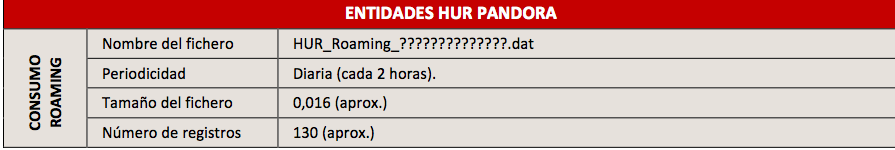
\includegraphics[width=14cm, keepaspectratio]{img/entidades5}
	  \caption{Entidades HUR Pandora}
	  \label{fig:entidades5}
	\end{figure}

	\item Bancos (BNK): desde los bancos se recibe la información relativa a las devoluciones de los recibos. Se reciben ficheros de diferentes bancos una vez al día y se procesan con la misma frecuencia. En la tabla de la figura~\ref{fig:entidades6} se muestran los detalles de los ficheros recibidos.

	\begin{figure}
	  \centering
	  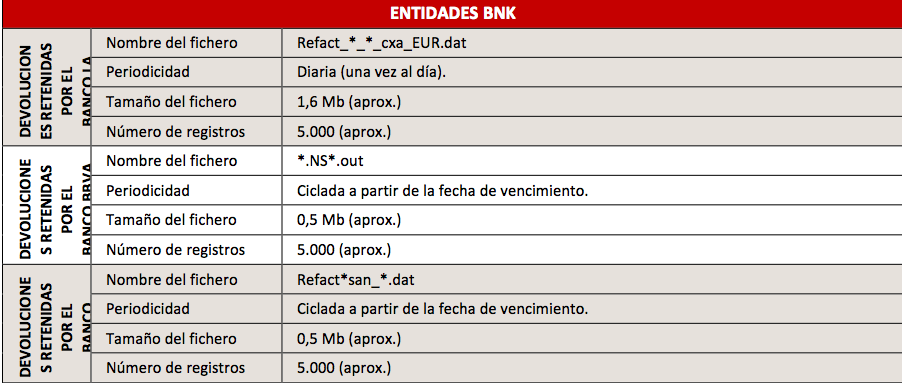
\includegraphics[width=14cm, keepaspectratio]{img/entidades6}
	  \caption{Entidades BNK}
	  \label{fig:entidades6}
	\end{figure}

	\item SAP: de SAP se recibe la información relativa a las devoluciones procesadas por este mismo sistema, así como los movimientos contables y la deuda. En las tablas de las figuras~\ref{fig:entidades7_1} y~\ref{fig:entidades7_2} se muestran los detalles de los ficheros recibidos.

	\begin{figure}
	  \centering
	  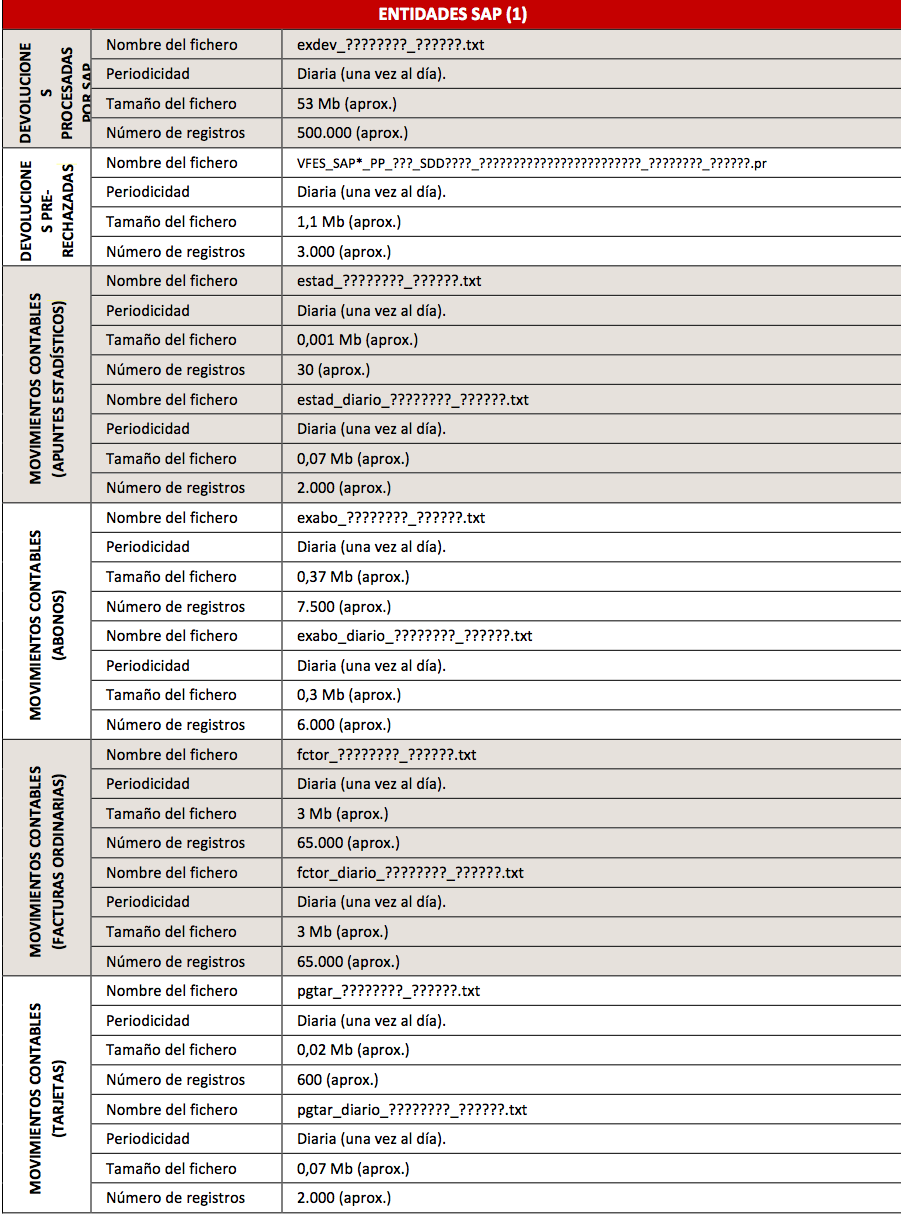
\includegraphics[width=14cm, keepaspectratio]{img/entidades7_1}
	  \caption{Entidades SAP (1)}
	  \label{fig:entidades7_1}
	\end{figure}

	\begin{figure}
	  \centering
	  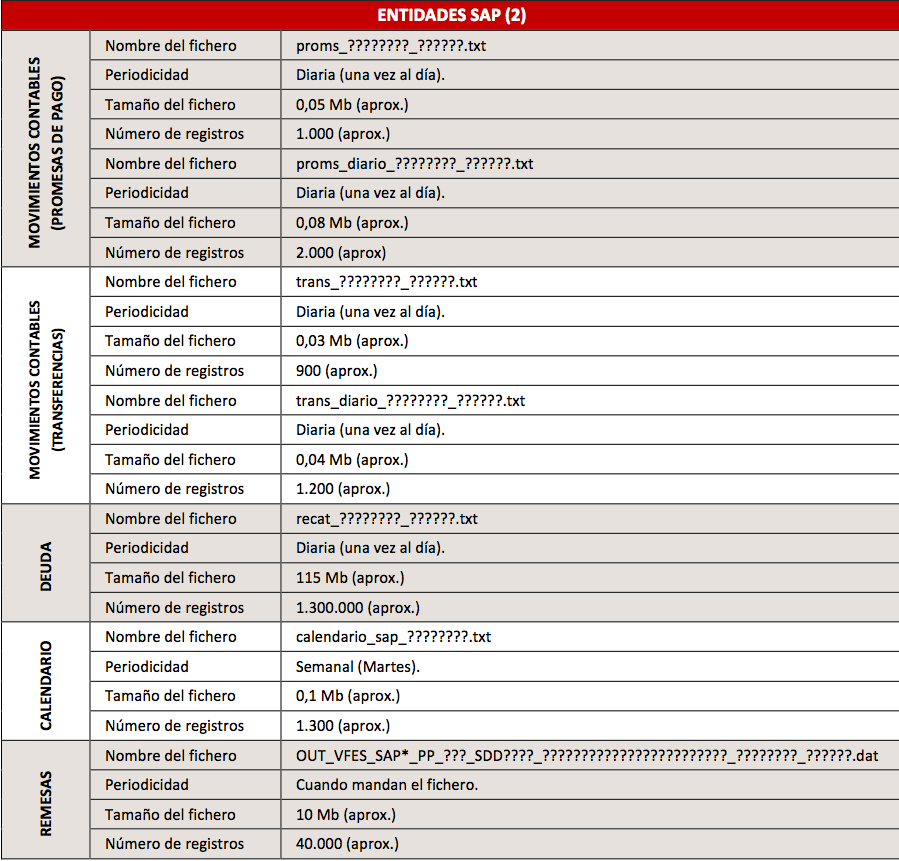
\includegraphics[width=14cm, keepaspectratio]{img/entidades7_2}
	  \caption{Entidades SAP (2)}
	  \label{fig:entidades7_2}
	\end{figure}
	
	\item Informa: se trata de una plataforma que ofrece información acerca de empresas; para este Datamart desde Informa llega la información de las empresas en situación concursal de forma semanal. En la tabla de la figura~\ref{fig:entidades8} se muestran los detalles del fichero recibido.

	\begin{figure}
	  \centering
	  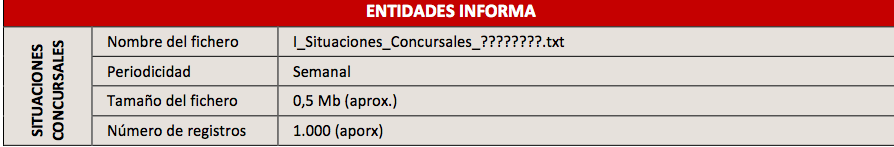
\includegraphics[width=14cm, keepaspectratio]{img/entidades8}
	  \caption{Entidades Informa}
	  \label{fig:entidades8}
	\end{figure}
	
	\item SEPA: desde SEPA se cargan las devoluciones procesadas por este sistema. En la tabla de la figura~\ref{fig:entidades9} se muestran los detalles del fichero recibido.

	\begin{figure}
	  \centering
	  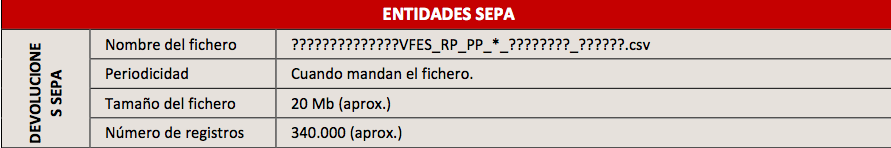
\includegraphics[width=14cm, keepaspectratio]{img/entidades9}
	  \caption{Entidades SEPA}
	  \label{fig:entidades9}
	\end{figure}
	
	\item Provisión Masiva. En la tabla de la figura~\ref{fig:entidades10} se muestran los detalles del fichero recibido.

	\begin{figure}
	  \centering
	  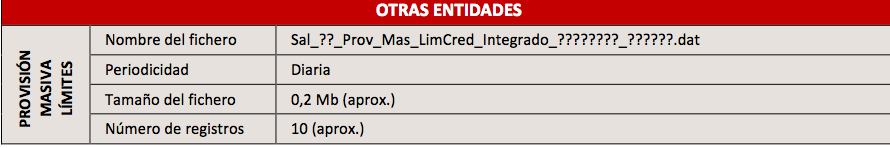
\includegraphics[width=14cm, keepaspectratio]{img/entidades10}
	  \caption{Entidades Otras}
	  \label{fig:entidades10}
	\end{figure}
	
	\item Asignaciones.
	
	\item Agex. Las agencias externas envían su cartera para su inclusión en el Datamart. En la tabla de la figura~\ref{fig:entidades11} se muestran los detalles del fichero recibido.

	\begin{figure}
	  \centering
	  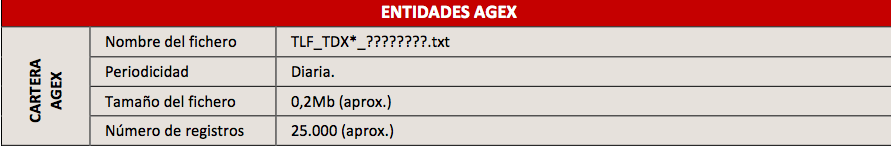
\includegraphics[width=14cm, keepaspectratio]{img/entidades11}
	  \caption{Entidades AGEX}
	  \label{fig:entidades11}
	\end{figure}
	
	\item Diccionarios. La información que se carga de Diccionarios es muy estática, es decir, no suele haber cambios de una ejecución a otra (se trata de tablas descriptivas). A pesar de ello, se reciben de manera diaria.
\end{itemize}

El sistema analítico del Datamart se procesa de manera ciclada, es decir, después de cada ciclo de facturación. La información del sistema analítico está en un esquema de la base de datos diferente al operacional. Las fuentes de entrada del sistema analítico son:
\begin{itemize}
	\item DWH: después de cada ciclo de facturación, desde el Datawarehouse se recibe en el Datamart de Riesgos la información de cartera, facturación, cambio de direcciones, promociones y llamadas pasarela.
	\item BO: desde BO se recibe la información correspondiente a la cartera y a los cobros. En la tabla de la figura~\ref{fig:entidades12} se muestran los detalles de los ficheros recibidos.

	\begin{figure}
	  \centering
	  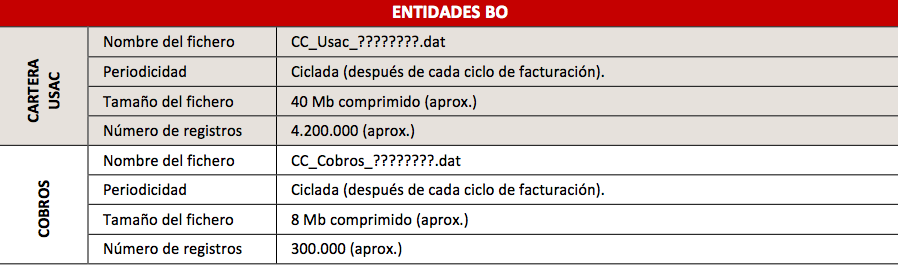
\includegraphics[width=14cm, keepaspectratio]{img/entidades12}
	  \caption{Entidades BO}
	  \label{fig:entidades12}
	\end{figure}
	
	\item Adquisiciones: desde Adquisiciones se recibe la información relativa a las solicitudes de alta, portabilidades, migraciones y cambios de titular, junto con una serie de indicadores. En la tabla de la figura~\ref{fig:entidades13} se muestran los detalles del fichero recibido.

	\begin{figure}
	  \centering
	  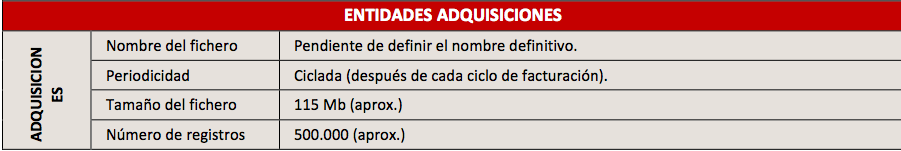
\includegraphics[width=14cm, keepaspectratio]{img/entidades13}
	  \caption{Entidades Adquisiciones}
	  \label{fig:entidades13}
	\end{figure}
\end{itemize}

En la figura ~\ref{fig:mapa_sistemas} se muestra un mapa de todos los sistemas de los que se extrae información para su procesado y tratamiento en el Datamart de Riesgos. Así mismo, se muestran los informes que el Datamart produce como salida y que se detallarán más adelante en este Proyecto.

\begin{figure}
  \centering
  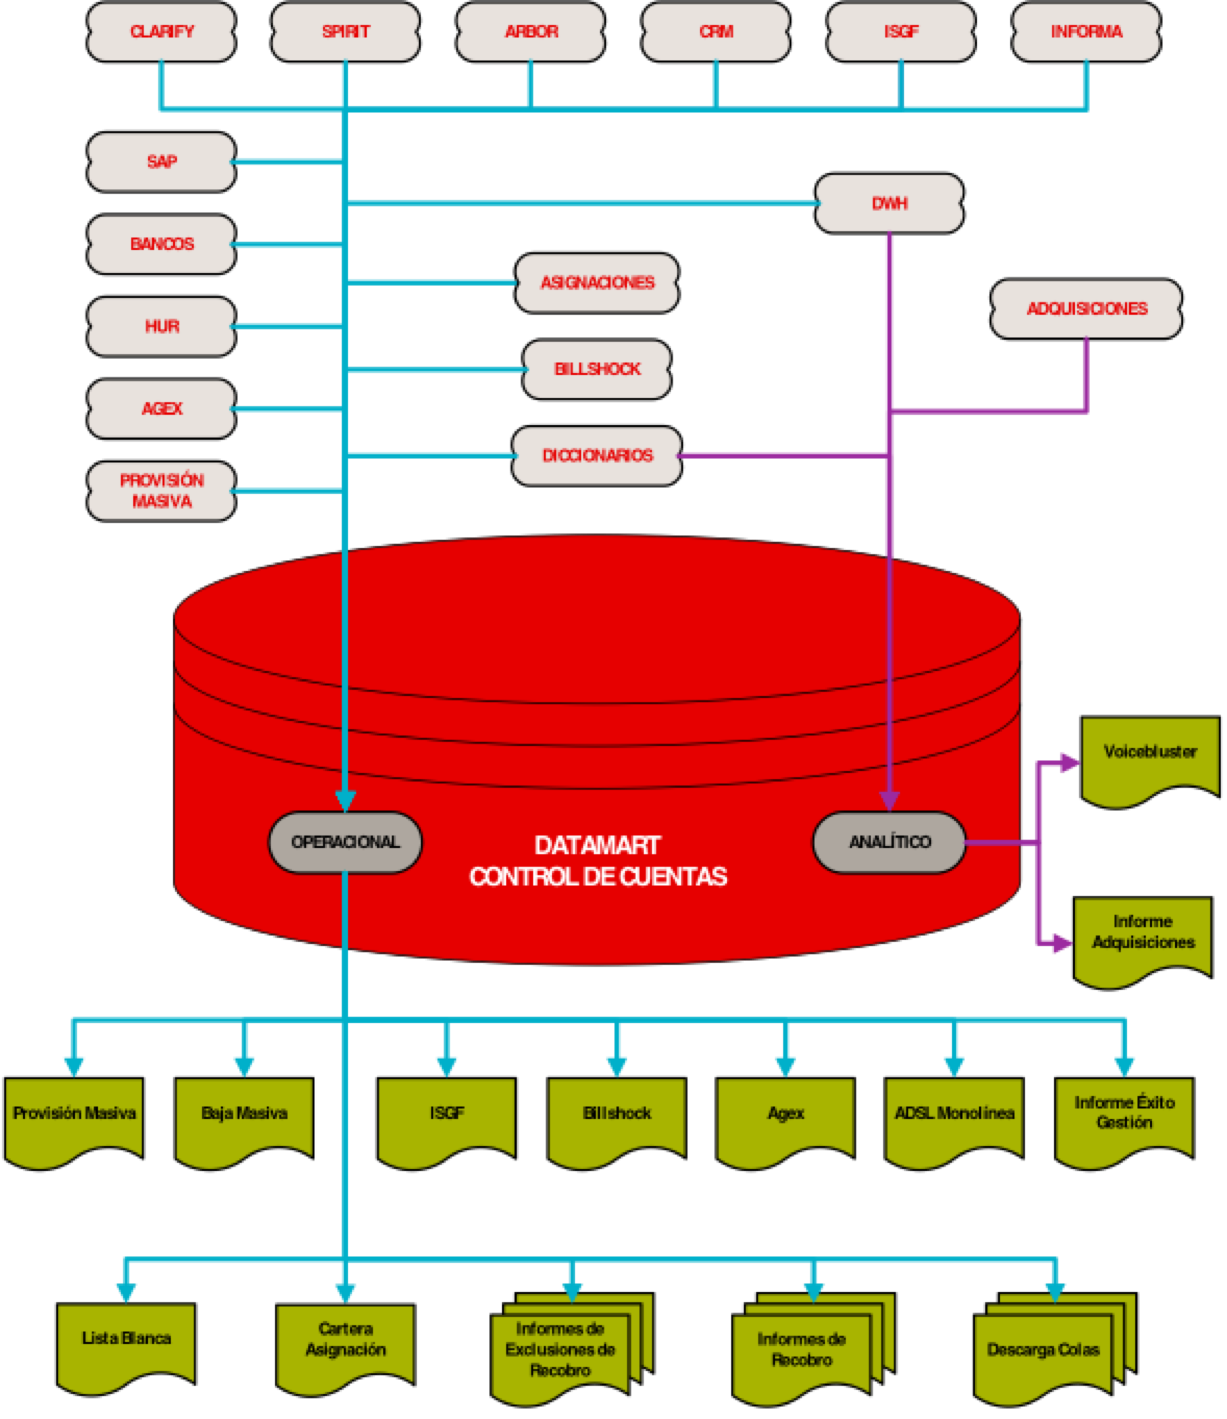
\includegraphics[width=15cm, keepaspectratio]{img/mapa_sistemas}
  \caption{Mapa de sistemas Datamart de riesgos}
  \label{fig:mapa_sistemas}
\end{figure}

\section{Monitorización de la ejecución} 
\label{sec:monitorizacion}
Para la monitorización diaria de las ejecuciones se dispone de un script que muestra la salida desde la propia línea de comandos. Este script lo que hace es comprobar los logs que generan los diferentes procesos: si alguno de los procesos no finaliza correctamente, en el correspondiente log aparecerá el error y este script mostrará por pantalla una alerta; del mismo modo, si los procesos periódicos no se han ejecutado cuando correspondía (por ejemplo, porque no han llegado los ficheros necesarios) también mostrará una alerta. Este script también refleja cuando un proceso se encuentra en ejecución.
Para ejecutar el script, nos conectaremos a la VPN mediante el Cliente VPN de Cisco, ejecutaremos PuTTy e iniciaremos sesión en la máquina UNIX. Para lanzar la ejecución del script, nos situaremos en la carpeta donde se encuentra mediante el comando \textit{cd} seguido de la carpeta y posteriormente ejecutaremos el script con \textit{ksh COMPROBAR\_EJECUCIONES}. En la figura ~\ref{fig:comprobar_ejecuciones} se muestra la salida por línea de comandos que proporciona este script.

\begin{figure}
  \centering
  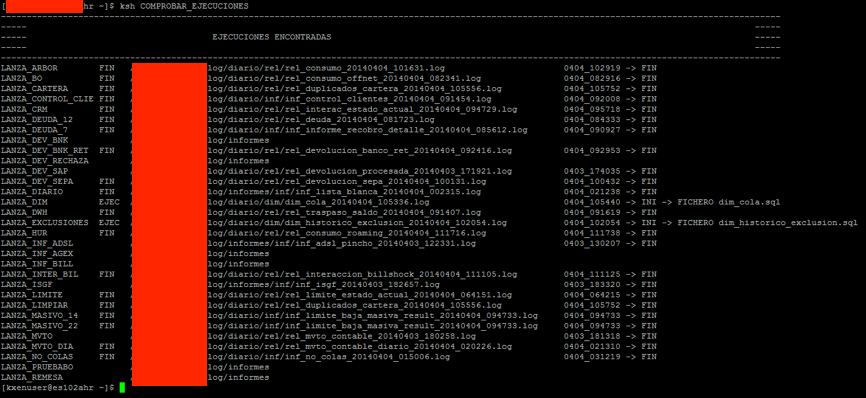
\includegraphics[width=15cm, keepaspectratio]{img/comprobar_ejecuciones}
  \caption{Salida por línea de comandos del script COMPROBAR\_EJECUCIONES}
  \label{fig:comprobar_ejecuciones}
\end{figure}

Los procesos los podemos diferenciar en aquellos cuya ejecución está programada y aquellos cuya ejecución se lleva a cabo bajo demanda. En los siguientes apartados se detallan los diferentes procesos, así como las cuestiones a tener en cuenta para el soporte y mantenimiento de los mismos.

\section{Ejecución programada de los procesos} 
\label{sec:ejecucion_programada}
Para controlar la ejecución programada hay que fijarse en la periodicidad de los diferentes procesos, ya que puede ser que se ejecuten una sola vez al día o varias. Para ello, existen dos ficheros de configuración en los cuales se lleva a cabo la planificación de los procesos: ./cfg/ctl\_lanzador.cfg y ./cfg/ctl\_planificador.cfg.

El lanzador, ctl\_lanzador.cfg, contiene los scripts que componen los lanzadores de tareas que se tienen que ejecutar, mientras que, en el planificador, ctl\_planificador.cfg, se configura la periodicidad y horas en las que estas tareas se ejecutan. Por ejemplo, en el fichero del planificador nos podemos encontrar una línea como la siguiente:
\begin{center}
	\textit{04\textbar00\textbar10\textbar08\textbar00\textbar/home/kxenuser/bin/LANZADOR-LANZA\_CARTERA}
\end{center}

Esto nos indica que el proceso LANZA\_CARTERA se empieza a ejecutar mediante el lanzador a las 04:00AM, comprobando si llega información nueva a sus respectivas carpetas cada 10 minutos. Si han llegado los ficheros, se ejecuta LANZA\_CARTERA y se procesan la información, en caso contrario, se sigue esperando hasta las 08:00AM.

En caso de que alguno de los procesos falle, se debe revisar el log de ejecución que se encuentra en ./log/FICHERO\_ERRORES\_LANZADOR. Aquí se puede identificar el fallo que se ha producido y, para analizar en detalle el error, se debe buscar el log del script concreto que falló en la ruta correspondiente.

Una vez localizado y resuelto el error y antes de relanzar el proceso, hay que eliminar el error del log FICHERO\_ERRORES\_LANZADOR, ya que el lanzador no permite ejecutar procesos que presentan error en dicho log. Una vez se ha limpiado el log de errores, se lanza por línea de comandos el proceso correspondiente:

\begin{center}
	\textit{nohup ksh LANZADOR ``LANZADOR QUE FALLÓ'' \&}
\end{center}

De cara a optimizar los recursos del Datamart, se deben comentar en el fichero ctl\_lanzador.cfg los scripts del proceso, dejando sin comentar únicamente el que falló y sus sucesores, volviendo a descomentarlos una vez haya finalizado para que no interfiera en sucesivas ejecuciones.

Por último, es importante tener en cuenta que algunos procesos dependen de otros, con lo que se debe controlar cuidadosamente la ejecución de aquellos procesos predecesores para que realicen sus tareas en plazo y no retrasen la ejecución del proceso dependiente.

\section{Ejecución bajo demanda de los procesos} 
\label{sec:ejecucion_demanda}
En el momento de realización de este proyecto se disponía de tres procesos que se ejecutaban bajo demanda. La monitorización de estos procesos también se lleva a cabo mediante el script COMPROBAR\_EJECUCIONES.

Para los procesos que se ejecutan bajo demanda es necesario que el solicitante nos remita el fichero a procesar. Al ser un proceso más manual que en el caso de ejecuciones programadas, es altamente recomendable, antes de procesar el fichero en cuestión, comprobar que nos lo envían con la información bien formada y con los campos correctos. Para ello, con el siguiente comando podemos detectar de una manera rápida si los campos son los adecuados:
\begin{center}
	\textit{head TLF\_TDX\_????????.txt}
\end{center}

\section{Fallos comunes en la ejecución diaria y tratamiento} 
\label{sec:fallos}

\begin{enumerate}
	\item Error en una tabla \par
En el caso de producirse algún error que afecte a alguna de las tablas que usan varios procesos, habrá que desplanificar la ejecución de dichos procesos para evitar un bucle de errores que afecte a más tablas del Datamart. 

Cuando tengamos que desplanificar algún proceso y luego queramos que se lance, lo volveremos a planificar con la hora actual (por ejemplo, si son las 14:00, en el planificador lo pondremos para que se lance a las 14:05). Habrá que tener especial cuidado al realizar esto, ya que el planificador a las 00:00 detiene todos los procesos y lee la planificación que haya configurada en ese momento. El problema radica en que, si tenemos algún proceso que tenga que estar ejecutándose continuamente, al replanificarlo a otra hora no se volverá a lanzar al día siguiente hasta esa hora. Para evitar esto, una vez se haya lanzado el proceso, en el planificador lo volvemos a cambiar para ponerlo a su hora original.

Ejemplo de uso: hay un problema en la tabla SERVICIOS\_V. Desplanificamos todas las tareas que usan este relacional hasta que solventemos el problema. Una vez solucionado, las volvemos a poner en el planificador con la hora actual + 5 minutos, y una vez se hayan lanzado, las volvemos a cambiar con la planificación original.

	\item Procesos con dependencias \par
	Como se ha indicado anteriormente, existen procesos que presentan dependencias con otros procesos. Esto queda reflejado en el fichero de configuración ctl\_dependencias.cfg, que contiene configuración como la siguiente:
	
\textit{LANZA\_EXCLUSIONES;pre\_exclusiones\_laborable.sh;LANZA\_DEUDA\_12;}

\begin{flushright}\textit{rel\_deuda.sh;0;36000}
\end{flushright}

\textit{LANZA\_EXCLUSIONES;pre\_exclusiones\_laborable.sh;LANZA\_CRM;}

\begin{flushright}\textit{rel\_interac\_estado\_actual.sh;0;36000}
\end{flushright}

\textit{LANZA\_EXCLUSIONES;pre\_exclusiones\_laborable.sh;LANZA\_CRM\_BO;}

\begin{flushright}\textit{rel\_interaccion\_cuenta\_cont.sh;0;36000}
\end{flushright}

\textit{LANZA\_EXCLUSIONES;pre\_exclusiones\_laborable.sh;LANZA\_MVTO\_DIA;}

\begin{flushright}\textit{rel\_mvto\_contable\_diario.sh;0;36000}
\end{flushright}

En este ejemplo, vemos que LANZA\_EXCLUSIONES depende de las tareas LANZA\_ DEUDA\_12, LANZA\_CRM, LANZA\_CRM\_BO y LANZA\_MVTO\_DIA. En concreto la dependencia consiste en que los scripts que ahí se indican se deben haber ejecutado correctamente en el día en el que se está intentando ejecutar LANZA\_EXCLUSIONES. Si fallase la ejecución de, por ejemplo, LANZA\_CRM\_BO, habría que seguir los siguientes pasos:
	\begin{itemize}
		\item Encontrar el fallo por el que la cadena CRM\_BO falló, solucionarlo y relanzar esta cadena.
		\item \textit{ksh ultima\_ejecucion\_correcta.sh LANZA\_EXCLUSIONES inf\_informe\_exclusion.sh}. El script ultima\_ejecucion\_correcta.sh lo que hace es forzar a que se detecte como correcta la ejecución de los scripts.
	\end{itemize}
	
	\item CRM \par
CRM es uno de los procesos que se ejecutan diariamente de forma programada. Este proceso lo que hace es cargar en el Datamart las interacciones que han tenido los clientes con el servicio de atención al cliente, categorizando esas interacciones en CASOS, SUBCASOS e INTERACCIÓN. Es habitual que la ejecución de este proceso falle debido a que los ficheros necesarios no llegan uno o varios días seguidos. A modo ilustrativo, a continuación se detallan los pasos que habría que seguir para solventar esta situación.

\begin{itemize}
	\item En primer lugar, una vez reclamados y obtenidos los ficheros, se dejan en la ruta de recepción correspondiente. Para el movimiento de ficheros podemos utilizar la línea de comandos a través de PuTTY o bien podemos utilizar la interfaz gráfica de FileZilla.
	\item A continuación, en el fichero de configuración del lanzador, ctl\_lanzador.cfg, se modificará la parte de LANZA\_CRM tal y como se muestra en la figura~\ref{fig:crm_fallos}, comentando todos los scripts pertenecientes a este proceso, excepto los scripts encargados de cargar los ficheros en tablas de \textit{staging}. En estas tablas se cargan los datos brutos de los ficheros.

\begin{figure}
  \centering
  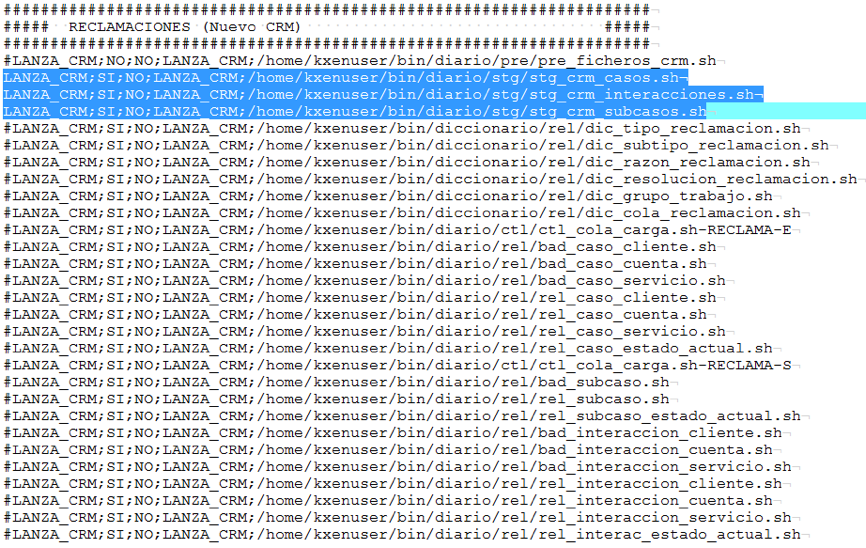
\includegraphics[width=14cm, keepaspectratio]{img/crm_fallos}
  \caption{Modificación fichero ctl\_lanzador.cfg para reprocesado de los ficheros del proceso CRM}
  \label{fig:crm_fallos}
\end{figure}

	\item Posteriormente, mediante línea de comandos ejecutamos el proceso con la instrucción \textit{nohup ksh LANZADOR LANZA\_CRM \&}.

	\item Una vez completado el proceso de carga de datos, comprobamos a través de Oracle que la información se ha cargado correctamente en las diferentes tablas de \textit{staging} (STG\_CRM\_CASOS, STG\_CRM\_SUBCASOS, STG\_CRM\_INTERACCIONES).

	\item Ahora habrá que borrar de los CASOS y los SUBCASOS la información un día posterior a la fecha del fichero no recibido, por ejemplo, si los ficheros del día 18 de mayo (con fecha del 17) no llegaron, habría que ejecutar lo siguiente en Oracle:

		\textit{delete from STG\_CRM\_SUBCASOS}
		
		\textit{where FECHA\_CIERRE is null;}
		
		\textit{delete from STG\_CRM\_SUBCASOS}
		
		\textit{where FECHA\_CREACION > = TO\_DATE('20140518', 'yyyymmdd');}
		
		\textit{delete from STG\_CRM\_CASOS}
		
		\textit{where FECHA\_CIERRE is null;}
		
		\textit{delete from STG\_CRM\_CASOS}


	\item Con este último paso eliminamos los casos posteriores a la fecha del fichero, que no interesa actualizar y los casos que no tuvieron cierre el día de no recepción del fichero. Nos quedamos con los casos cerrados el día del fichero, se hayan creado ese día o no. Del \textit{staging} de interacciones no se elimina nada porque todo son altas nuevas, así que se hace un volcado completo de la información del fichero al relacional.
	
	\item Volvemos al fichero ctl\_lanzador.cfg y comentamos de manera inversa, es decir, comentamos los scripts que cargan en \textit{staging} y descomentamos el resto de scripts. Por último, desde línea de comandos ejecutamos el lanzador igual que la primera vez.
\end{itemize}
El proceso realizado aquí para corregir este error producido por la ausencia de ficheros es una tipología, pudiendo encontrarnos con otras, como por ejemplo que los ficheros de entrada del proceso contengan información malformada o con duplicados, etc. No existe una forma general de solucionar los problemas que se puedan presentar en el Datamart y, por ello, no se abordan en este proyecto, ya que dependerá de la manera en la que el proceso esté diseñado, en los sistemas de información de entrada (cada sistema ofrece la información de una manera, por ejemplo, unos sistemas pueden enviar información con la vista de un solo día, o con la información histórica) y también depende de las necesidades y consideraciones que el área de negocio tenga. 
\end{enumerate}

\section{Ejemplo de proceso: LANZA\_EXCLUSIONES} 
\label{sec:lanza_exclusiones}
En este apartado se va a explicar el funcionamiento de uno de los procesos del Datamart de riesgos, para lo que se ha seleccionado el proceso de LANZA\_EXCLUSIONES.

El proceso de exclusiones se emplea para no tener en cuenta a aquellos clientes con deuda pendiente de abonar y que no se deben tener en cuenta para solicitar su recobro. Entre los motivos para excluir a un cliente están los siguientes:

\begin{itemize}
	\item Reclamación oficial: marcado en la legislación vigente, no se debe solicitar al cliente ningún cobro de deuda. Este es el tipo de reclamación más importante a tener en cuenta y por la que el proceso completo resulta vital, ya que si la organización se pusiese en contacto con un cliente para reclamar una deuda pendiente de cobro, dicho cliente podría iniciar acciones judiciales contra la organización.
	
	\item Reclamación no oficial: se puede decidir proteger a un cliente por otros motivos más allá de los legales (por ejemplo, que se esté haciendo un recálculo de la cuota a pagar por el cliente).
\end{itemize}

Para dar soporte y mantener adecuadamante este proceso, lo más importante es tener en cuenta los ficheros de entrada de los que depende el proceso, así como el resto de procesos de los que depende. Por otro lado, es importante tener en cuenta los plazos definidos para recibir los ficheros de entrada y el \textit{deadline} marcado para haber ejecutado el proceso y enviar el informe correspondiente.

En concreto, este proceso tiene una fuerte dependencia del proceso LANZA\_CRM, el cual se encarga de cargar y procesar en el Datamart la información relativa a las interacciones realizadas por los clientes con los \textit{Call Center}. Por ello, una de las tareas más importantes es la de asegurar la ejecución y finalización del proceso LANZA\_CRM antes del comienzo de LANZA\_EXCLUSIONES. En caso de error en LANZA\_CRM habrá que solucionarlo manualmente cuanto antes si fuese por un error en el procesado, ya que si el error se debe a que no han llegado los ficheros necesarios para LANZA\_CRM, lo único que podremos hacer es reclamarlos e informar del retraso en los informes de LANZA\_EXCLUSIONES.

Otra de las tareas llevadas a cabo en relación a este proceso consistía en la exclusión de clientes bajo demanda. Para ello, mediante Oracle y a través de \textit{queries} SQL, se modificaban las tablas en las que se volcaban los resultados del proceso LANZA\_EXCLUSIONES para incluir a los nuevos clientes excluidos bajo demanda y, posteriormente, se ejecutaba únicamente la parte del proceso en la que se generaban los informes a partir de estas tablas.


\section{Rendimiento y optimización del Datamart} 
\label{sec:rendimiento}
Uno de los aspectos importantes y, en ocasiones olvidado debido al trabajo operativo del día a día, es el de mantener un buen rendimiento en el Datamart, evitando sobrecargas que puedan provocar la caída del sistema.

Para ello, resulta de vital importancia revisar y mantener una adecuada planificación de los procesos, evaluando la carga que suponen cada uno de ellos y programando su ejecución de manera que no se solapen varios procesos que sobrecarguen el Datamart.

Del mismo modo, es importante mantener unos procesos eficientes. Este es un aspecto controvertido, ya que en las organizaciones se trabaja en equipos multidisciplinares y con gran número de personas, y no suele existir una única manera correcta de hacer las cosas. La manera de mantener unos procesos eficientes es revisarlos manualmente en busca de comandos innecesarios en los scripts o queries de SQL muy complejas e ineficientes.

Para evaluar el coste de las instrucciones SQL, Oracle cuenta con una utilidad la cual, sin necesidad de ejecutar la query sobre el Datamart, nos evalúa el coste. Con esto nos podemos hacer una idea de la carga que supondrá para el Datamart y, o bien diseñar una query menos costosa para llevar a cabo la misma tarea o, si esto no fuese posible, tenerlo en cuenta a la hora de ejecutar el proceso en el que se encuentre el script que contenga la query en cuestión.

Además de mantener una adecuada planificación, de cara a optimizar el uso del Datamart y evitar bloqueos del mismo, es de vital importancia prestar atención al espacio de almacenamiento, tanto de las máquinas que soportan el Datamart como de la propia estructura y del espacio libre de cada uno de los esquemas de la base de datos.

En este Datamart conseguimos liberar grandes cantidades de espacio en disco de la máquina UNIX trasladando a otra máquina todos aquellos archivos ya procesados y logs de una antigüedad superior a dos años. Por otro lado, se llevó a cabo una profunda revisión de las tablas de cada uno de los esquemas de la base de datos. Como resultado de esta revisión, se borraron aquellas tablas que habían dejado de usarse por diferentes motivos (principalmente, porque se crean y mejoran procesos y se dejan de usar otros, dejando de usar las tablas asignadas a estos).

Además, se llevó a cabo la racionalización en el uso de tablas auxiliares y de pruebas, ya que en algunos casos se llegaban a hacer copias íntegras de las tablas que más información almacenaban solamente para llevar a cabo alguna prueba. Para hacernos una idea, estamos hablando de tablas que en el entorno productivo podían rondar en 10\% de la capacidad de almacenamiento dedicado a la base de datos, con lo que si se habían hecho dos copias completas por dos de los analistas del equipo, se podía llegar a ocupar una parte importante del espacio.

%%%%%%%%%%%%%%%%%%%%%%%%%%%%%%%%%%%%%%%%%%%%%%%%%%%%%%%%%%%%%%%%%%%%%%%%%%%%%%%%
%%%%%%%%%%%%%%%%%%%%%%%%%%%%%%%%%%%%%%%%%%%%%%%%%%%%%%%%%%%%%%%%%%%%%%%%%%%%%%%%
% RESULTADOS %
%%%%%%%%%%%%%%%%%%%%%%%%%%%%%%%%%%%%%%%%%%%%%%%%%%%%%%%%%%%%%%%%%%%%%%%%%%%%%%%%

%\cleardoublepage
%\chapter{Resultados}
%Los resultados de este proyecto, al tratarse de una colaboración en un proyecto en curso, son los %obtenidos de la consecución y ejecución de las tareas de soporte y mantenimiento del Datamart de %riesgos. Estos objetivos y tareas son los descritos en el capítulo~\ref{chap:objetivos} y la %consecución de los mismos se describe en el capítulo~\ref{chap:conclusiones}.

%%%%%%%%%%%%%%%%%%%%%%%%%%%%%%%%%%%%%%%%%%%%%%%%%%%%%%%%%%%%%%%%%%%%%%%%%%%%%%%%
%%%%%%%%%%%%%%%%%%%%%%%%%%%%%%%%%%%%%%%%%%%%%%%%%%%%%%%%%%%%%%%%%%%%%%%%%%%%%%%%
% CONCLUSIONES %
%%%%%%%%%%%%%%%%%%%%%%%%%%%%%%%%%%%%%%%%%%%%%%%%%%%%%%%%%%%%%%%%%%%%%%%%%%%%%%%%

\cleardoublepage
\chapter{Conclusiones}
\label{chap:conclusiones}

\section{Consecución de objetivos}
\label{sec:consecucion-objetivos}

El objetivo principal de este proyecto es el de conocer el funcionamiento de un Datamart, las tareas necesarias para dar soporte a su operativa y el mantenimiento del mismo, habiendo sido ampliamente cubierto.

En cuanto a los objetivos secundarios descritos en el capítulo~\ref{chap:objetivos}, todos ellos fueron cubiertos al 100\%, debido a que dichos objetivos formaban parte de las tareas de las cuales yo era el responsable.


\section{Aplicación de lo aprendido}
\label{sec:aplicacion}

La Licenciatura en Ingeniería de Telecomunicación me ha ofrecido una formación completa, partiendo desde el estudio y entendimiento de los fundamentos, hasta el desarrollo de las habilidades necesarias para dar solución a problemas que, a primera vista, pueden resultar diferentes de todo lo visto con anterioridad. En el ámbito de este proyecto, la formación y conocimientos aplicados más relevantes han sido aquellos adquiridos en las asignaturas del ámbito de la programación, redes y administración y configuración de sistemas. Algunas de las asignaturas con mayor impacto en estas áreas de conocimiento han sido:

\begin{enumerate}
	\item \textbf{Fundamentos de la programación.} Esta asignatura ofrece las bases y el conocimiento básico sobre la programación, permitiendo desarrollar buenos hábitos a la hora de programar y comprender las estructuras más simples y su manejo.
	\item \textbf{Métodos de programación.} De igual forma que en el caso anterior, esta asignatura sentó las bases sobre el uso de procedimientos y funciones en la programación.
	\item \textbf{Fundamentos de los computadores (I y II).} En ambas asignaturas, igual que en las anteriores, se nos presentaron los conocimientos básicos acerca de la computación, tanto a nivel software como hardware. Tanto los conocimientos como la terminología aprendida en estas asignaturas resulta fundamental para desenvolvernos con soltura en un entorno dominado por las Tecnologías de la Información.
	\item \textbf{Sistemas Telemáticos (I y II).} Estas son, sin duda, las asignaturas cuyos conocimientos se aplican en mayor medida durante este proyecto. Todos aquellos conocimientos adquiridos en estas asignaturas y relacionado con la gestión de entornos UNIX mediante línea de comandos resultó fundamental para un buen aprovechamiento de la colaboración.
	\item \textbf{Servicios y aplicaciones telemáticas.} Desde el punto de vista más técnico, esta asignatura nos pone en contacto por vez primera con \textit{Python}, lo cual me resultó útil durante la colaboración para mejorar pequeñas herramientas y programas de los que disponía para operar el Datamart.
	\item \textbf{Sistemas de Tiempo Real.} Los conocimientos adquiridos en esta asignatura fueron de gran ayuda para el desarrollo de este proyecto, sobre todo los relacionados con la planificación de procesos y la gestión de dependencias.
	\item \textbf{Proyectos.} Por último, esta asignatura ofrece los conocimientos básicos que cualquier profesional debe tener. Toda la terminología relacionada con la gestión de proyectos, las habilidades necesarias para hacer presentaciones en público, capacidad de toma de decisión en entornos dinámicos y los riesgos asociados a esa toma de decisión son conceptos clave para entender el funcionamiento de cualquier organización.
\end{enumerate}

Además de los conocimientos adquiridos en las asignaturas cursadas, durante la doble titulación he adquirido habilidades y aptitudes que también me han ayudado a desenvolverme en un entorno profesional. Entre otras, capacidad de defender mis propias ideas y propuestas, capacidad de análisis y sentido crítico, orientación a resultados, ...

\section{Lecciones aprendidas}
\label{sec:lecciones_aprendidas}

En el ámbito más técnico, la realización de este proyecto me ha permitido adquirir un conocimiento más profundo de las capacidades de los \textit{Shell scripts}, dado que la gestión de las máquinas que soportan el propio Datamart se lleva a cabo casi al completo a través de ellos. Por otro lado, durante el proyecto he aprendido a manejar con soltura bases de datos, analizando la información del Datamart mediante \textit{queries} SQL y optimizando la ejecución de los procesos encargados de dar tratamiento a la información del Datamart y de la generación de informes.

El haber colaborado en un proyecto de \textit{Business Intelligence} me ha dotado de la visión de la importancia de la buena gestión de los datos para las compañías, además de ser consciente del enorme volumen de información que manejan las organizaciones con las que nos relacionamos las personas en nuestro día a día.

En cuanto a habilidades y conocimientos generales, el haber colaborado en un proyecto real con un cliente al otro lado me ha permitido obtener una visión y orientación a resultados y a satisfacción de cliente que me ha permitido crecer profesionalmente. Esto mismo me ha permitido mejorar mis habilidades en cuanto a comunicación con otros equipos de trabajo, así como el escalado de problemas o situaciones complicadas a los superiores.

\section{Trabajos futuros}
\label{sec:trabajos_futuros}

Como modelo ideal hacia el que debería orientarse el Datamart de riesgos, se propone migrar todas las funcionalidades implementadas a través de procesos que se ejecutan mediante \textit{scripts} hacia un entorno de BI que permita optimizar las tareas a la hora de analizar información. Para ello, se podría migrar hacia un entorno implementado en R, el cual es un entorno y lenguaje de programación enfocado hacia el análisis estadístico de los datos.

Por otro lado, aunque se trata de una tarea continuación de lo que ya se venía haciendo, debido a la continua evolución de las necesidades de negocio, resulta imprescindible continuar con la optimización de los actuales procesos.


%%%%%%%%%%%%%%%%%%%%%%%%%%%%%%%%%%%%%%%%%%%%%%%%%%%%%%%%%%%%%%%%%%%%%%%%%%%%%%%%
%%%%%%%%%%%%%%%%%%%%%%%%%%%%%%%%%%%%%%%%%%%%%%%%%%%%%%%%%%%%%%%%%%%%%%%%%%%%%%%%
% APÉNDICE(S) %
%%%%%%%%%%%%%%%%%%%%%%%%%%%%%%%%%%%%%%%%%%%%%%%%%%%%%%%%%%%%%%%%%%%%%%%%%%%%%%%%

%\cleardoublepage
%\appendix
%\chapter{Manual de usuario}
%\label{app:manual}


%%%%%%%%%%%%%%%%%%%%%%%%%%%%%%%%%%%%%%%%%%%%%%%%%%%%%%%%%%%%%%%%%%%%%%%%%%%%%%%%
%%%%%%%%%%%%%%%%%%%%%%%%%%%%%%%%%%%%%%%%%%%%%%%%%%%%%%%%%%%%%%%%%%%%%%%%%%%%%%%%
% BIBLIOGRAFIA %
%%%%%%%%%%%%%%%%%%%%%%%%%%%%%%%%%%%%%%%%%%%%%%%%%%%%%%%%%%%%%%%%%%%%%%%%%%%%%%%%

\cleardoublepage

% Las siguientes dos instrucciones es todo lo que necesitas
% para incluir las citas en la memoria
\bibliographystyle{abbrv}
\bibliography{memoria}  % memoria.bib es el nombre del fichero que contiene
% las referencias bibliográficas. Abre ese fichero y mira el formato que tiene,
% que se conoce como BibTeX. Hay muchos sitios que exportan referencias en
% formato BibTeX. Prueba a buscar en http://scholar.google.com por referencias
% y verás que lo puedes hacer de manera sencilla.
% Más informaciÛn: 
% http://texblog.org/2014/04/22/using-google-scholar-to-download-bibtex-citations/

\end{document}
